\chapter{Design}
\label{chap:design}
AlGa is implemented in Flutter. This makes it possible to study the UI having in mind also the logic of the application, with the result of a highly user-focused interface.
In particular, we tried to stick to Google Material Design guidelines. 

When we had to decide between beauty and clarity, we chose clarity. This is a key element, because mobile users can very impatient. The possibility to install and uninstall apps in very little time makes it fundamental for developers to "capture" their users from the very first look.

Complex UIs can create confusion and users may find the app unpleasant to deal with. So, simplicity was one of our key value for the design of AlGa.

In the next section, some design choices are presented with their motivations.

\section{Icon}
Also the icon (shown in Figure~\ref{fig:icon}) has been designed keeping in mind the principles suggested by Google for what concerns applications' icons.
In particular the icon has been drawn by Paolo Razzino, a friend and collaborator external to the group.
\begin{figure}[h]
    \centering
    
\includegraphics[scale=0.5]{Pics/icon.png}
    \caption{AlGa's icon.}
    \label{fig:icon}
\end{figure}
Its elements are a lightning, symbol of electric energy, which obviously recall the nature of the electric vehicles involved in the app; then an green alga (seaweed) which recalls the green and environmental element of electric vehicles adoption. Moreover, it's also an acronym for "Alessandro" and "Guelfi".
The shape is squared, as suggested by Google guidelines; its look, simple and modern, is appealing also when shown in a black and white notification (Figure~\ref{fig:icon_bw}).
\begin{figure}[H]
    \centering
    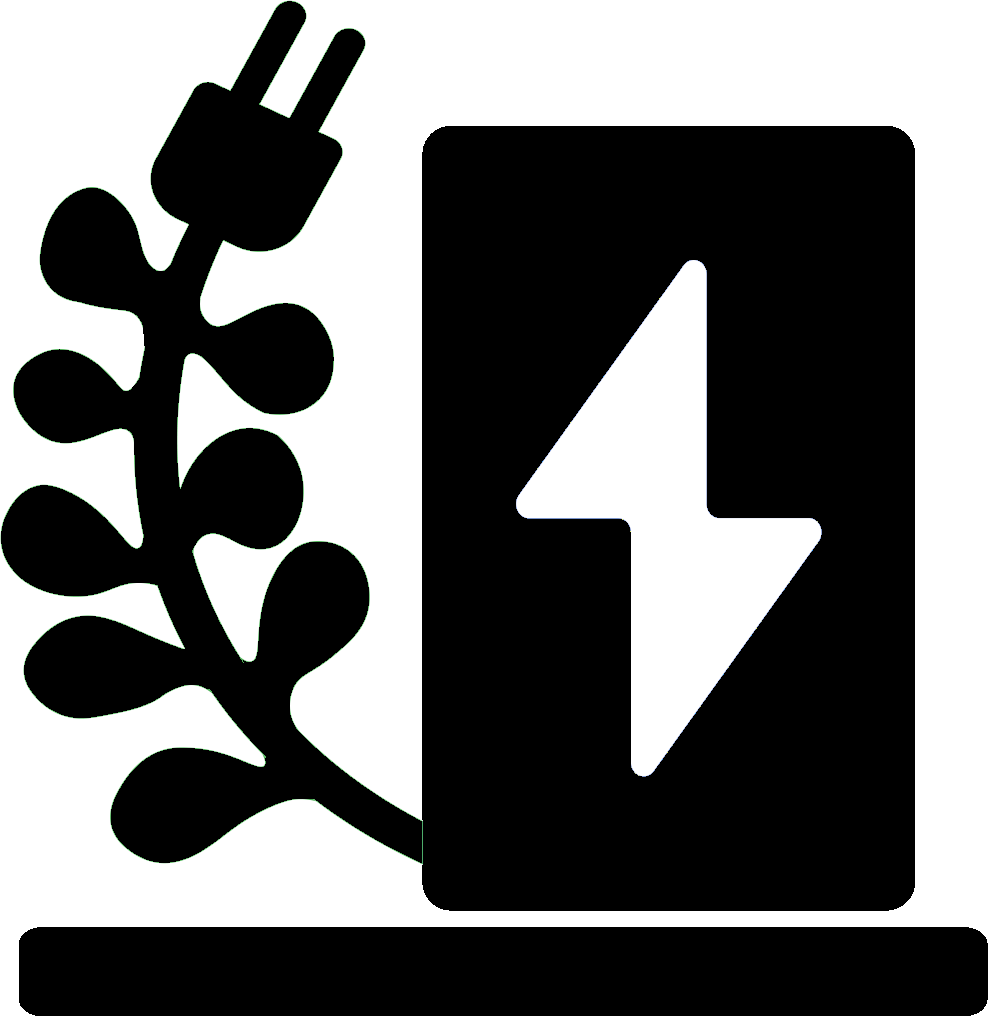
\includegraphics[scale=0.5]{Pics/icon_bw.png}
    \caption{AlGa's icon in black and white version.}
    \label{fig:icon_bw}
\end{figure}

\section{Navigation}
To let the user navigate inside the application, we chose to implement a Tab selector.
A Tab selector is a navigation element which provides some buttons on the bottom of the screen, where each button corresponds to a single screen.
This option is suggested by the Material Design rules if the sections are from 2 to 5. Given that, in our case, three screens are needed, this is a shoehorn case.

\section{Stats}
The statistics screen is made to be minimal but still useful. First of all, we thought what could be the values that an user may want to check which are also available to a mobile application.
We decided that, we the help of notifications and an user input, the total amount of cash spent, the kW recharged and the mean price for kW could be useful metrics.

As we can see in Figure~\ref{fig:stats}a, the three metrics are preceded by a selector which can be set on "Week", "Month" and "Year". This way the user can select a grade of granularity better suited for their goal (for example: how many kW I recharged this month?). 

However, given that the user may make some recharges without using AlGa, or some collected recharges may be uncorrect, we added the possibility to manually modify or add recharges. In Figure~\ref{fig:stats}b the user can create a new recharge selecting the date and hour, the cash spent and the kW recharged. In Figure~\ref{fig:stats}c the user is modifying an existing recharge, in order to correct some wrong values.

\begin{figure}[H]
    \centering
    \subfloat[]
	{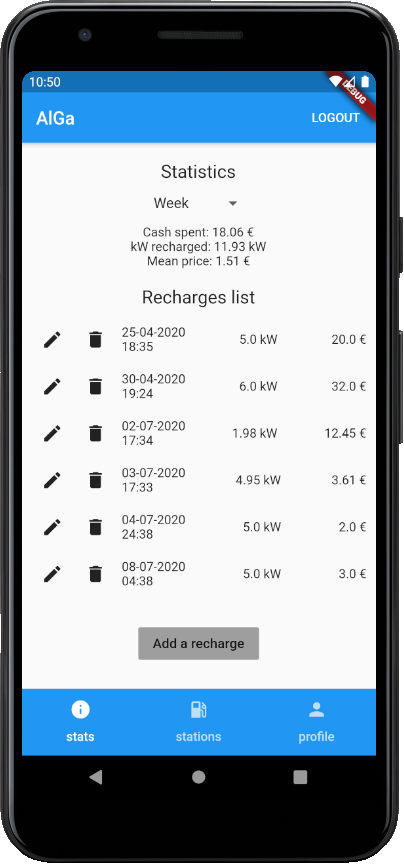
\includegraphics[width=0.3\linewidth]{Pics/MockUps/Stats.png}}\quad
    \subfloat[]
	{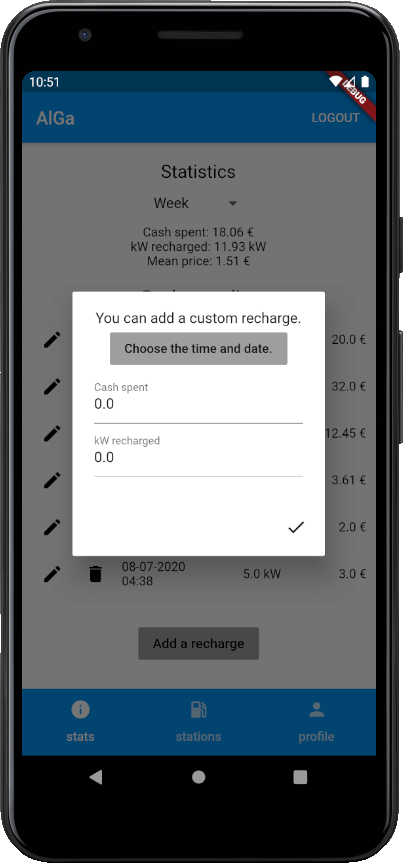
\includegraphics[width=0.3\linewidth]{Pics/MockUps/Stats2.png}}\quad
    \subfloat[]
	{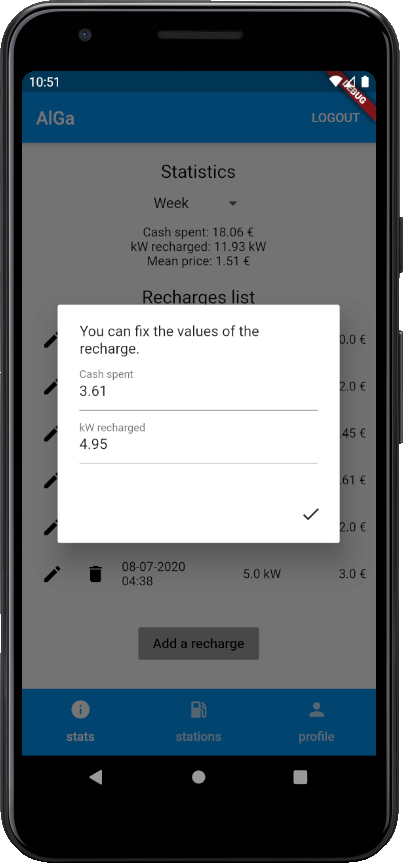
\includegraphics[width=0.3\linewidth]{Pics/MockUps/Stats3.png}}\quad
    \caption{Screenshots of the Stats screen.}
    \label{fig:stats}
\end{figure}

\section{Stations}
The Stations screen is, probably, the most important one of the application. The users can look for the recharge stations for their car on a map provided by Google Maps.
The common operations of moving, zoom, centering on user location and compass are offered by the Flutter plugin for Google Maps; our work was to create the custom pins for the stations.

As we can see in Figure~\ref{fig:stations}a recharge stations are marked with an icon created ad-hoc for AlGa (shown in Figure~\ref{fig:stations_markers}) The color of the icon refers to the availability of the station: green means that the stations has free places, red otherwise.

\begin{figure}[H]
    \centering
    \subfloat[]
	{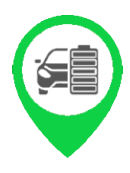
\includegraphics[width=0.2\linewidth]{Pics/station_green.png}}\quad
    \subfloat[]
	{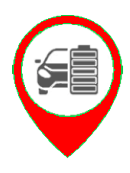
\includegraphics[width=0.2\linewidth]{Pics/station_red.png}}\quad
    \caption{Recharge stations markers.}
    \label{fig:stations_markers}
\end{figure}

Users can use a swipe panel in which stations are displayed and ordered according to three criteria: price, speed and distance (Figure~\ref{fig:stations}b).
This way the user can look for the more fit station, given that details of every station are presented in a simple and convenient place. Moreover, from the same panel, users can click on the "locate" button in order to highlight the station on the map, or they can click on the "GO" button which will open a Google Maps trip toward that station.

Lastly, users can also inspect the details of a station by just clicking over it (Figure~\ref{fig:stations}c). A little window, reachable with the thumb, appears and displays the distance, price and speed of the recharge stations. Again, users can start the navigation for that particular station using the "GO" button.

\begin{figure}[H]
    \centering
    \subfloat[]
	{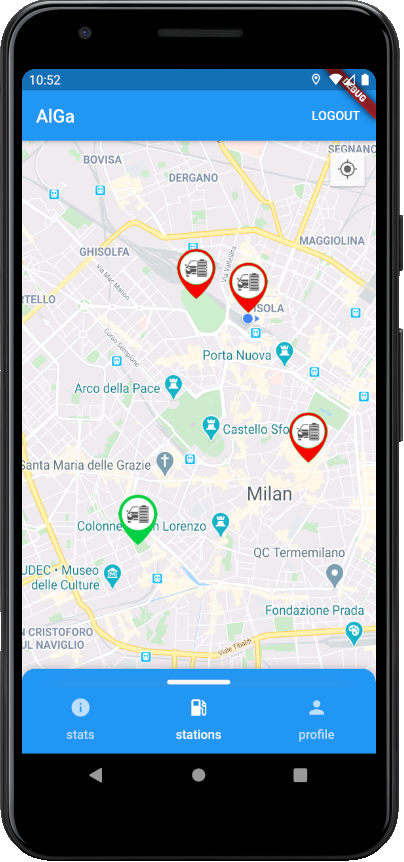
\includegraphics[width=0.3\linewidth]{Pics/MockUps/Stations.png}}\quad
    \subfloat[]
	{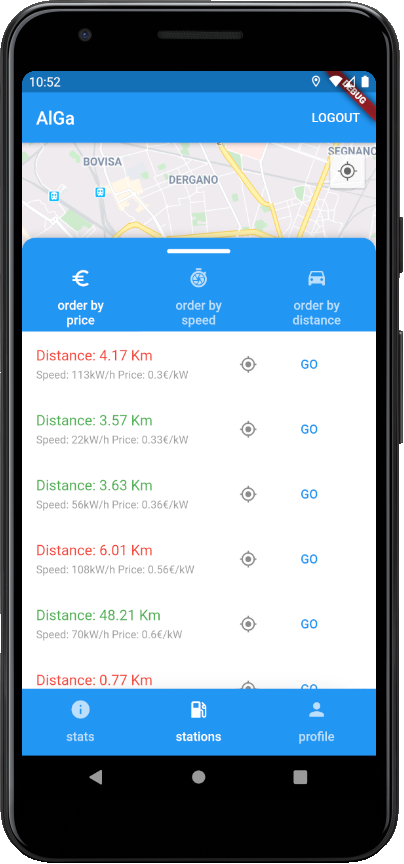
\includegraphics[width=0.3\linewidth]{Pics/MockUps/Stations2.png}}\quad
    \subfloat[]
	{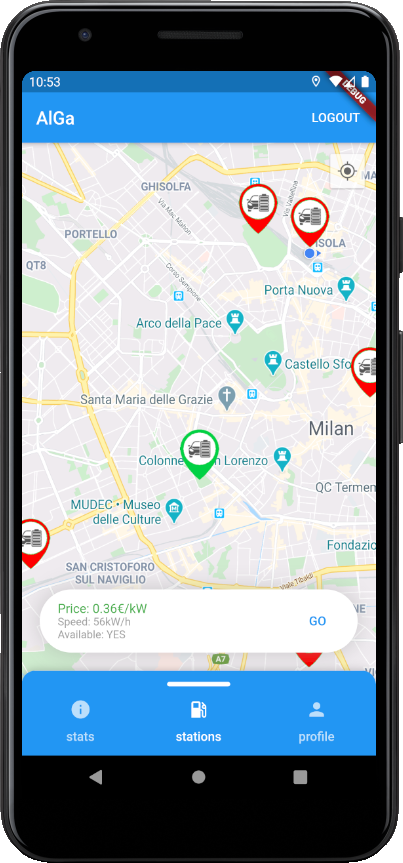
\includegraphics[width=0.3\linewidth]{Pics/MockUps/Stations3.png}}\quad
    \caption{Screenshots of the Stations screen.}
    \label{fig:stations}
\end{figure}

\newpage
\section{Profile}
The more classic screen is the profile one. From this screen users can modify their attributes like nickname, e-mail and password.
Initially, an overview is presented (Figure~\ref{fig:profile}a. The data is fetched directly from the database and rendered in the widgets.

A profile pic can be optionally set; a click on the "camera" button will trigger the default Android file selector which will let the user choose an image from their memory.
In Figure~\ref{fig:profile}b we see an example of profile modification: the user wants to change their username. To do so, a window with a validating form (in order to prevent the user from submitting incompatible content) is shown. The user has just to select a new name and to click the tick button.

Lastly, the user can also modify their car. This is important because the value of battery and range are used to provide statistics about the recharges. As we can see in Figure~\ref{fig:profile}c, users can either select a pre-defined car from a list (fetched from the database) of just select the "Custom" options and, then, manually set the battery and range values.

\begin{figure}[H]
    \centering
    \subfloat[]
	{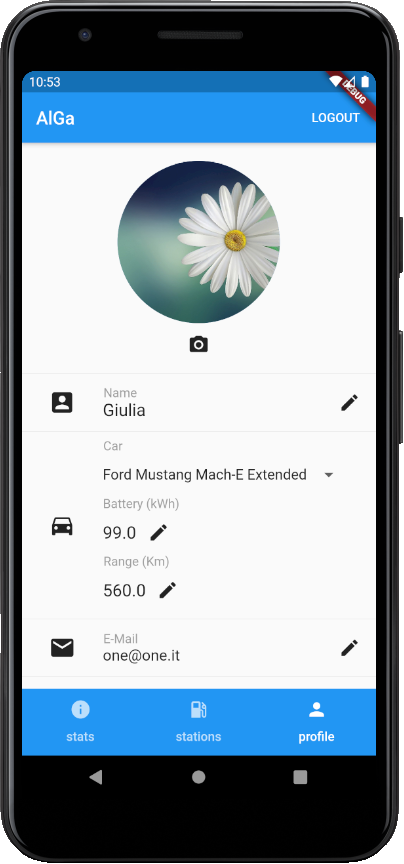
\includegraphics[width=0.3\linewidth]{Pics/MockUps/Profile.png}}\quad
    \subfloat[]
	{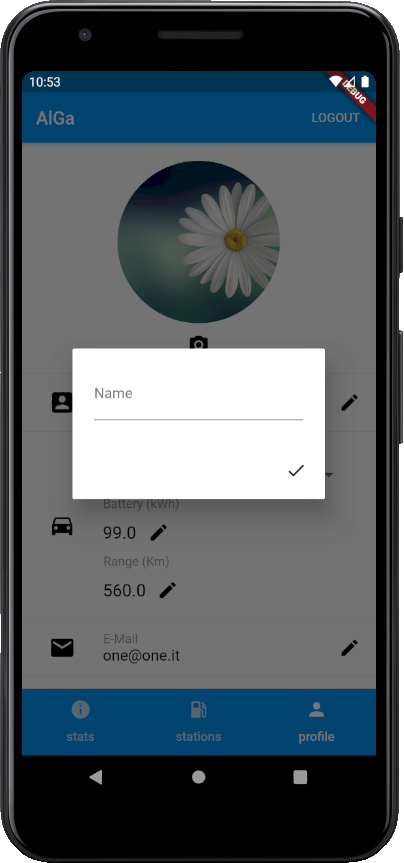
\includegraphics[width=0.3\linewidth]{Pics/MockUps/Profile2.png}}\quad
    \subfloat[]
	{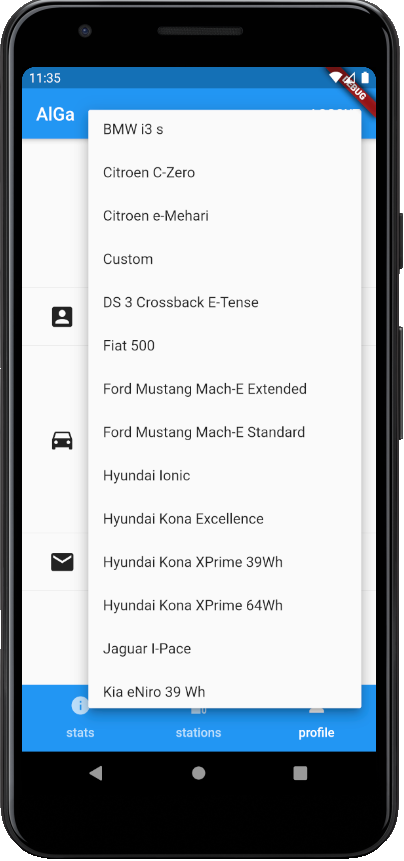
\includegraphics[width=0.3\linewidth]{Pics/MockUps/Profile3.png}}\quad
    \caption{Screenshots of the Profile screen.}
    \label{fig:profile}
\end{figure}

